\documentclass{article}
	\usepackage{graphicx}

	\begin{document}

	\title{HW/SW Entwurfssprachen am Beispiel System-C}
	\author{Florian Zaruba, Thomas Weber}

	\maketitle

	%\begin{abstract}
	%The abstract text goes here.
	%\end{abstract}

	\section{HW/SW Design Languages}
	\subsection{Motivation}
	The primary driver leading to the need for a new system design language is the same that previously lead to the need for the current design languages: increasing design complexity.
	
	Modern electronic systems consist of many sub-systems and components, but we will focus primarily on hardware, software, and algorithms. In modern systems, each of these disciplines has become more complex. Likewise, the interaction has become increasingly complex.
	Interactions imply that trade offs between the domains are becoming more important for meeting customer requirements. System development teams find themselves asking questions like, “Should this function be implemented in hardware, software, or with a better algorithm?” Systems are so complex, just deriving specifications from customer requirements has become a daunting task.
	
	Increasing number of embedded devices significantly stresses the topic of what should be implemented in HW and what in SW. To be resource efficient is a key aspect of an embedded design.
	
	\begin{itemize}
		\item Abstraction
		\item Design reuse
		\item Team discipline
		\item project reuse
		\item Automation    
	\end{itemize}
	
	
	SW leverages all aspects while hardware is stuck on a relatively low abstraction layer (RTL - Level) and focuses on the other 4 aspects.
	\subsection{SDL}
	The key goal is now to find an appropiate abstraction level between HW and SW (algorithms) which possibly can describe both equally good.  
		
	The underlying concept of TLM is to model only the level of detail that is needed by the engineers developing the system components and sub- system for a particular task in the development process. By modeling only the necessary details, design teams can realize huge gains in modeling speed thus enabling a new methodology. At this level, changes are relatively easy because the development team has not yet painted itself into a corner with low-level details such as a parallel bus implementation versus a serial bus implementation (a classical top down approach).
	
	Using TLMs makes tasks usually reserved for hardware implementations practical to run on a model early in the system development process. TLM is a concept independent of language. However, to implement and refine TLM models, it is helpful to have a language like SystemC whose features support independent refinement of functionality and communication that is crucial to efficient TLM development.
	
	Some of the refinemand tasks can even be automated.
	
	[JPEG example]
		
	Advantage for software: TLM allows an early model of software. It is simulated along with the hardware model and gets cross compiled to the specific arichtecture.
	
	At the 2010 DVCon event, OSCI produced a specification of the first synthesizable subset of SystemC for industry standardization.
	
	Alternatives:
	\begin{itemize}
		\item SystemC - by accelera systems initiative
		\item SpecC - ANSI C programming language. By Embedded Computer Systems at University of California, Irvine in 2001 - used mainly in Japan. SpecC is more simplictic. Architectural model maps directly to silicon.
		\item System Verilog - Extension of classical verilog with verification.
	\end{itemize}
	
	
	\section{What is SystemC}
	SystemC is a High Level Abstraction Language which aims to combine the benefits of hardware description languages and software.
	
	Hardware description languages have the big advantage that they are very performant.
	They execute exactly this operations for which they are designed for.	
	Software that runs on a processor is relatively easy to read and can be, in contrast to HDL, easy  tested and verified.	
	The long compilation process of the hardware modules and the design cycle which is very time consuming, hence the whole partitioning procedure had to be passed, make a better solution desirable.
	Furthermore hardware cannot be easily tested and verified and it cannot be updated\footnote{Except over an JTAG interface, in configurable chips like FPGAs}.
	
	SystemC shortens the design cycle because it makes it possible to write hardware and software in one language.
	It is an additional library to C/C++ which is mostly used in context of embedded systems today.
	The SystemC modules can be compiled in hardware and the C/C++ program which uses this modules fits best on the chip hence both components are tested together.
	  \subsection{History}
	  ARM Ltd., CoWare, Synopsys and CynApps teamed up to develop SystemC (CynApps later became Forte Design Systems) to launch it first draft version in 1999.
	  
	   At this time it provided some basic features, e.g., structural hierarchy and connectivity, clock-cycle accuracy, delta cycles, four-valued logic (0, 1, X, Z), and bus-resolution functions.
		
	    It was also possible to break down designs it into modules in order to reuse code.
	    
	    SystemC 2.0 was started in the late 2000. It extends the previous version with events as primitive behavior triggers as well as channels, interfaces and ports.
		
	    It was also more powerful in modeling at transaction level.
	    Furthermore its complete library were new coded to upgrade it to an independent System Level Description Language (SLDL).
		
		 The (Language Reference Manual) LRM provides the definitive statement of the semantics of SystemC.
		 
		 OSCI also provide an open-source proof-of-concept simulator (sometimes incorrectly referred to as the reference simulator), which can be downloaded from the OSCI website.[2] Although it was the intent of OSCI that commercial vendors and academia could create original software compliant to IEEE 1666, in practice most SystemC implementations have been at least partly based on the OSCI proof-of-concept simulator.
		 
		\subsection{Comparison}
		Several languages have emerged to address the various aspects of system design. Although Ada and Java have proven their value, C/C++ is predominately used today for embedded system software. The hardware description languages (HDLs), VHDL and Verilog, are used for simulating and synthesizing digital circuits. Vera and e are the languages of choice for functional verification of complex application-specific integrated circuits (ASICs). SystemVerilog is a new language that evolves the Verilog language to address many hardware-oriented system design issues. Matlab and several other tools and languages such as SPW and System Studio are widely used for capturing system requirements and developing signal processing algorithms.
		
	  \subsection{Benefits}
	  
	  tba
	  
	  \subsection{Drawbacks}
	  
	  tba
	  
	  \subsection{Features}
	  SystemC contains a lot of features like (logical) datatypes, modules, processes/threads, ports, signals or the time which is very important in context of an System Level Modelling language.
	   \begin{itemize}
 	    \item{Datatypes}
 	    \item{Modules}
 	    \item{Processes/Threads}
 	    \item{Ports and Signals}
  	    \item{Time}
	   \end{itemize}
	  \subsection{SysC vs. C vs VHDL}
	  See presentation.
	\section{Partitioning}

	
	  \subsection{What is Partitioning?}
	  Partitioning means the separation of hardware and software parts with focus on hardware/software co-design.
	  Traditionally the hardware part of an embedded system is written in VHDL \textit{(more present in Europe)} or Verilog \textit{(more present in the USA)} while the software part is written in \textit{assembly}, \textit{C} or \textit{C++}.
	  The common design-flow (depicted in Figure~\ref{fig:flow}) shows that partitioning splits the design in hardware and software.
	  The software part is the shorter one of this two paths because it needs only an compiler to translate it to machine-code. Therefore, the hardware part is the much longer way because of the hardware design-flow which is necessary for every chip-design.
	    \begin{figure}[h]
	      \centering
	      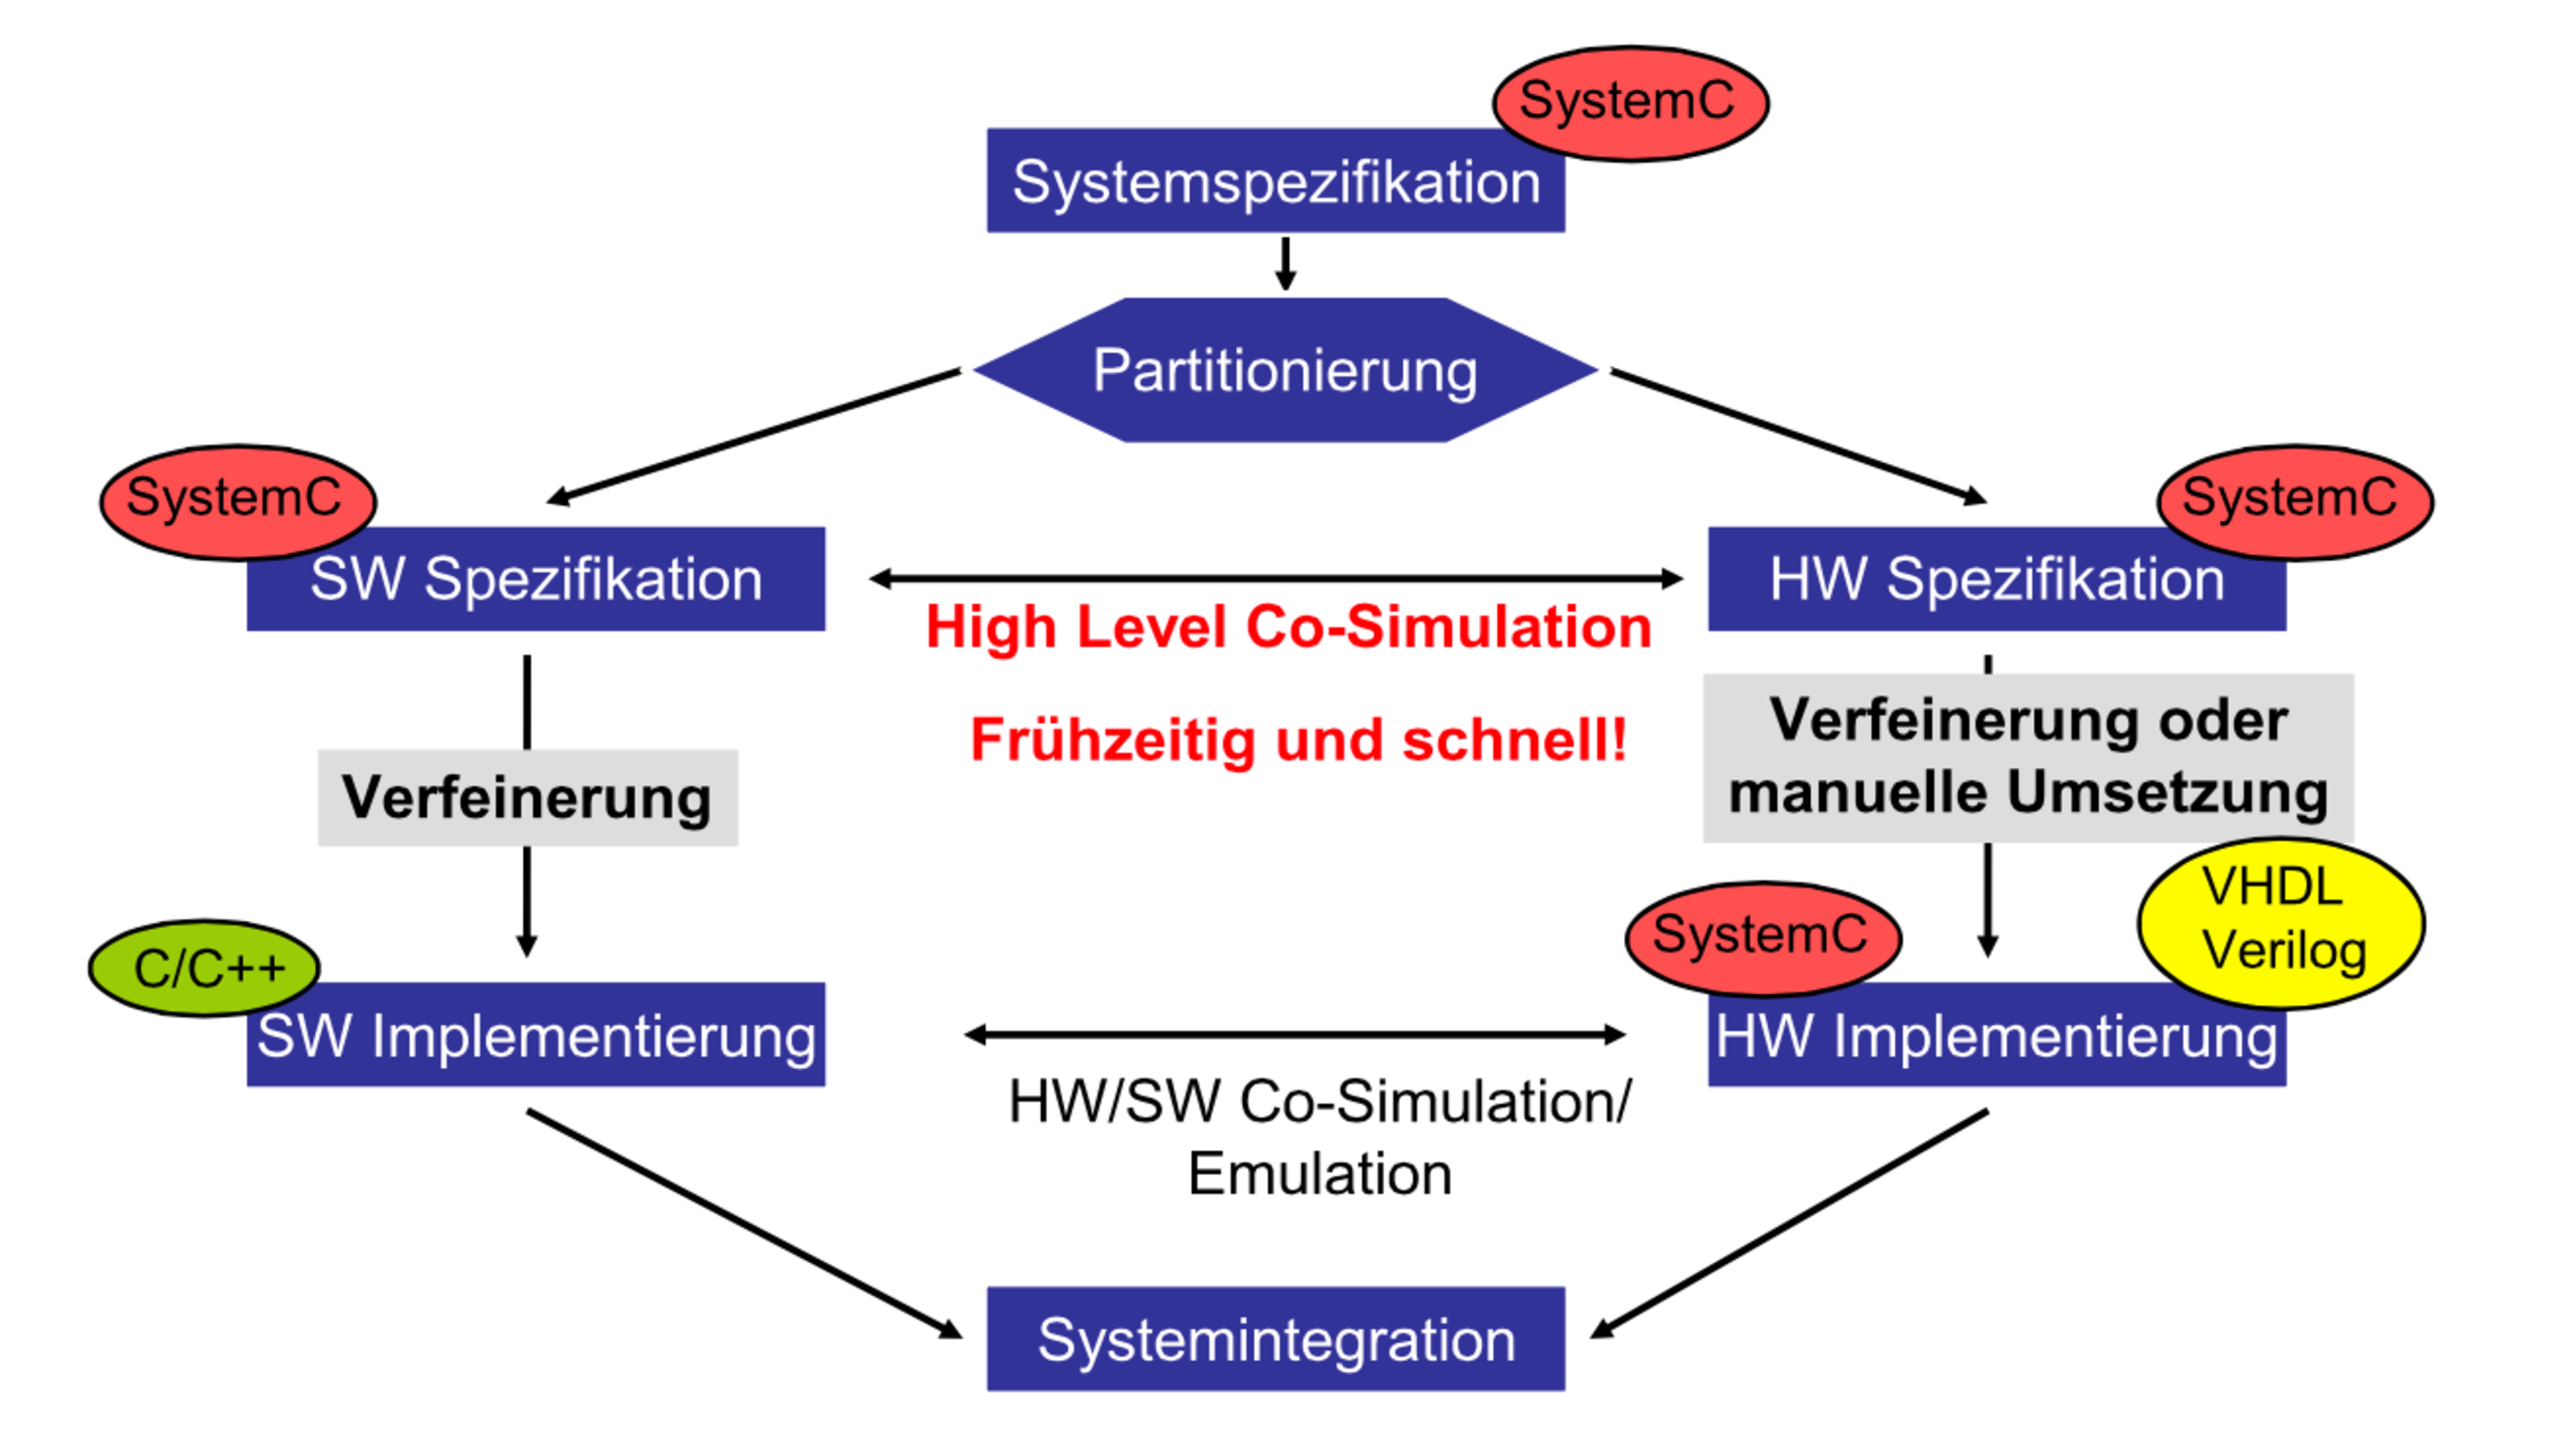
\includegraphics[scale=0.18]{../pictures/design_flow.pdf}
	      \caption{Design flow in context with SystemC.}
	      \label{fig:partitioning_sysc}
	    \end{figure}  
	  If the hardware and software parts should be modified because of, e.g., performance reasons, these two parts must be modified or completely redesigned in order to fit the specifications.
	  This leads to an much higher and probably expensive procedure for the hardware part, thus its design-flow is much longer and every change in the \textit{VHDL/Verilog} code leads to a new compilation, technology-mapping and place and route. %	  Unless there are other circumstances, the \textit{system definition} and the \textit{specification} steps are part of the project management which have to be done only once.
	
	\section{Automation of Partitioning}
	  
	  Design Space Exploration - simulate many different impementations which are possible. There are user given constraints (hardware effort, software effort, timing...).
	  \subsection{Partitioning Algorithms}
	    There exist partitioning algorithms which can be adjusted over constraints.
	    These algorithms use graph theory (Discrete Mathematics VO/UE) among other techniques.
	    Examples for algorithms: \\
	     \texttt{Kernighan-Lin-Algorithm}\\
	     \texttt{Simulated annealing}(Algorithmen und Datenstrukturen 2 VU)
	     
	  \subsection{Design Space Exploration}
	    
	  
	\section{Tools}	  
	  \subsection{LegUP}
	  LegUP\footnote{Its current version is 3.0} is an open source high level synthesis tool for FPGA based systems from the University of Toronto. 
	  It takes an standart C program as input and implements the hardware fitting part to hardware and the software fitting part to software.
	  LegUP uses an MIPS soft core and uses a standard bus interface for communication between the hardware parts and the processor.  
	  \textbf{Automatic Partitioning? - Yes in a way.}
	  
	    \begin{figure}[hp]
	      \centering
	      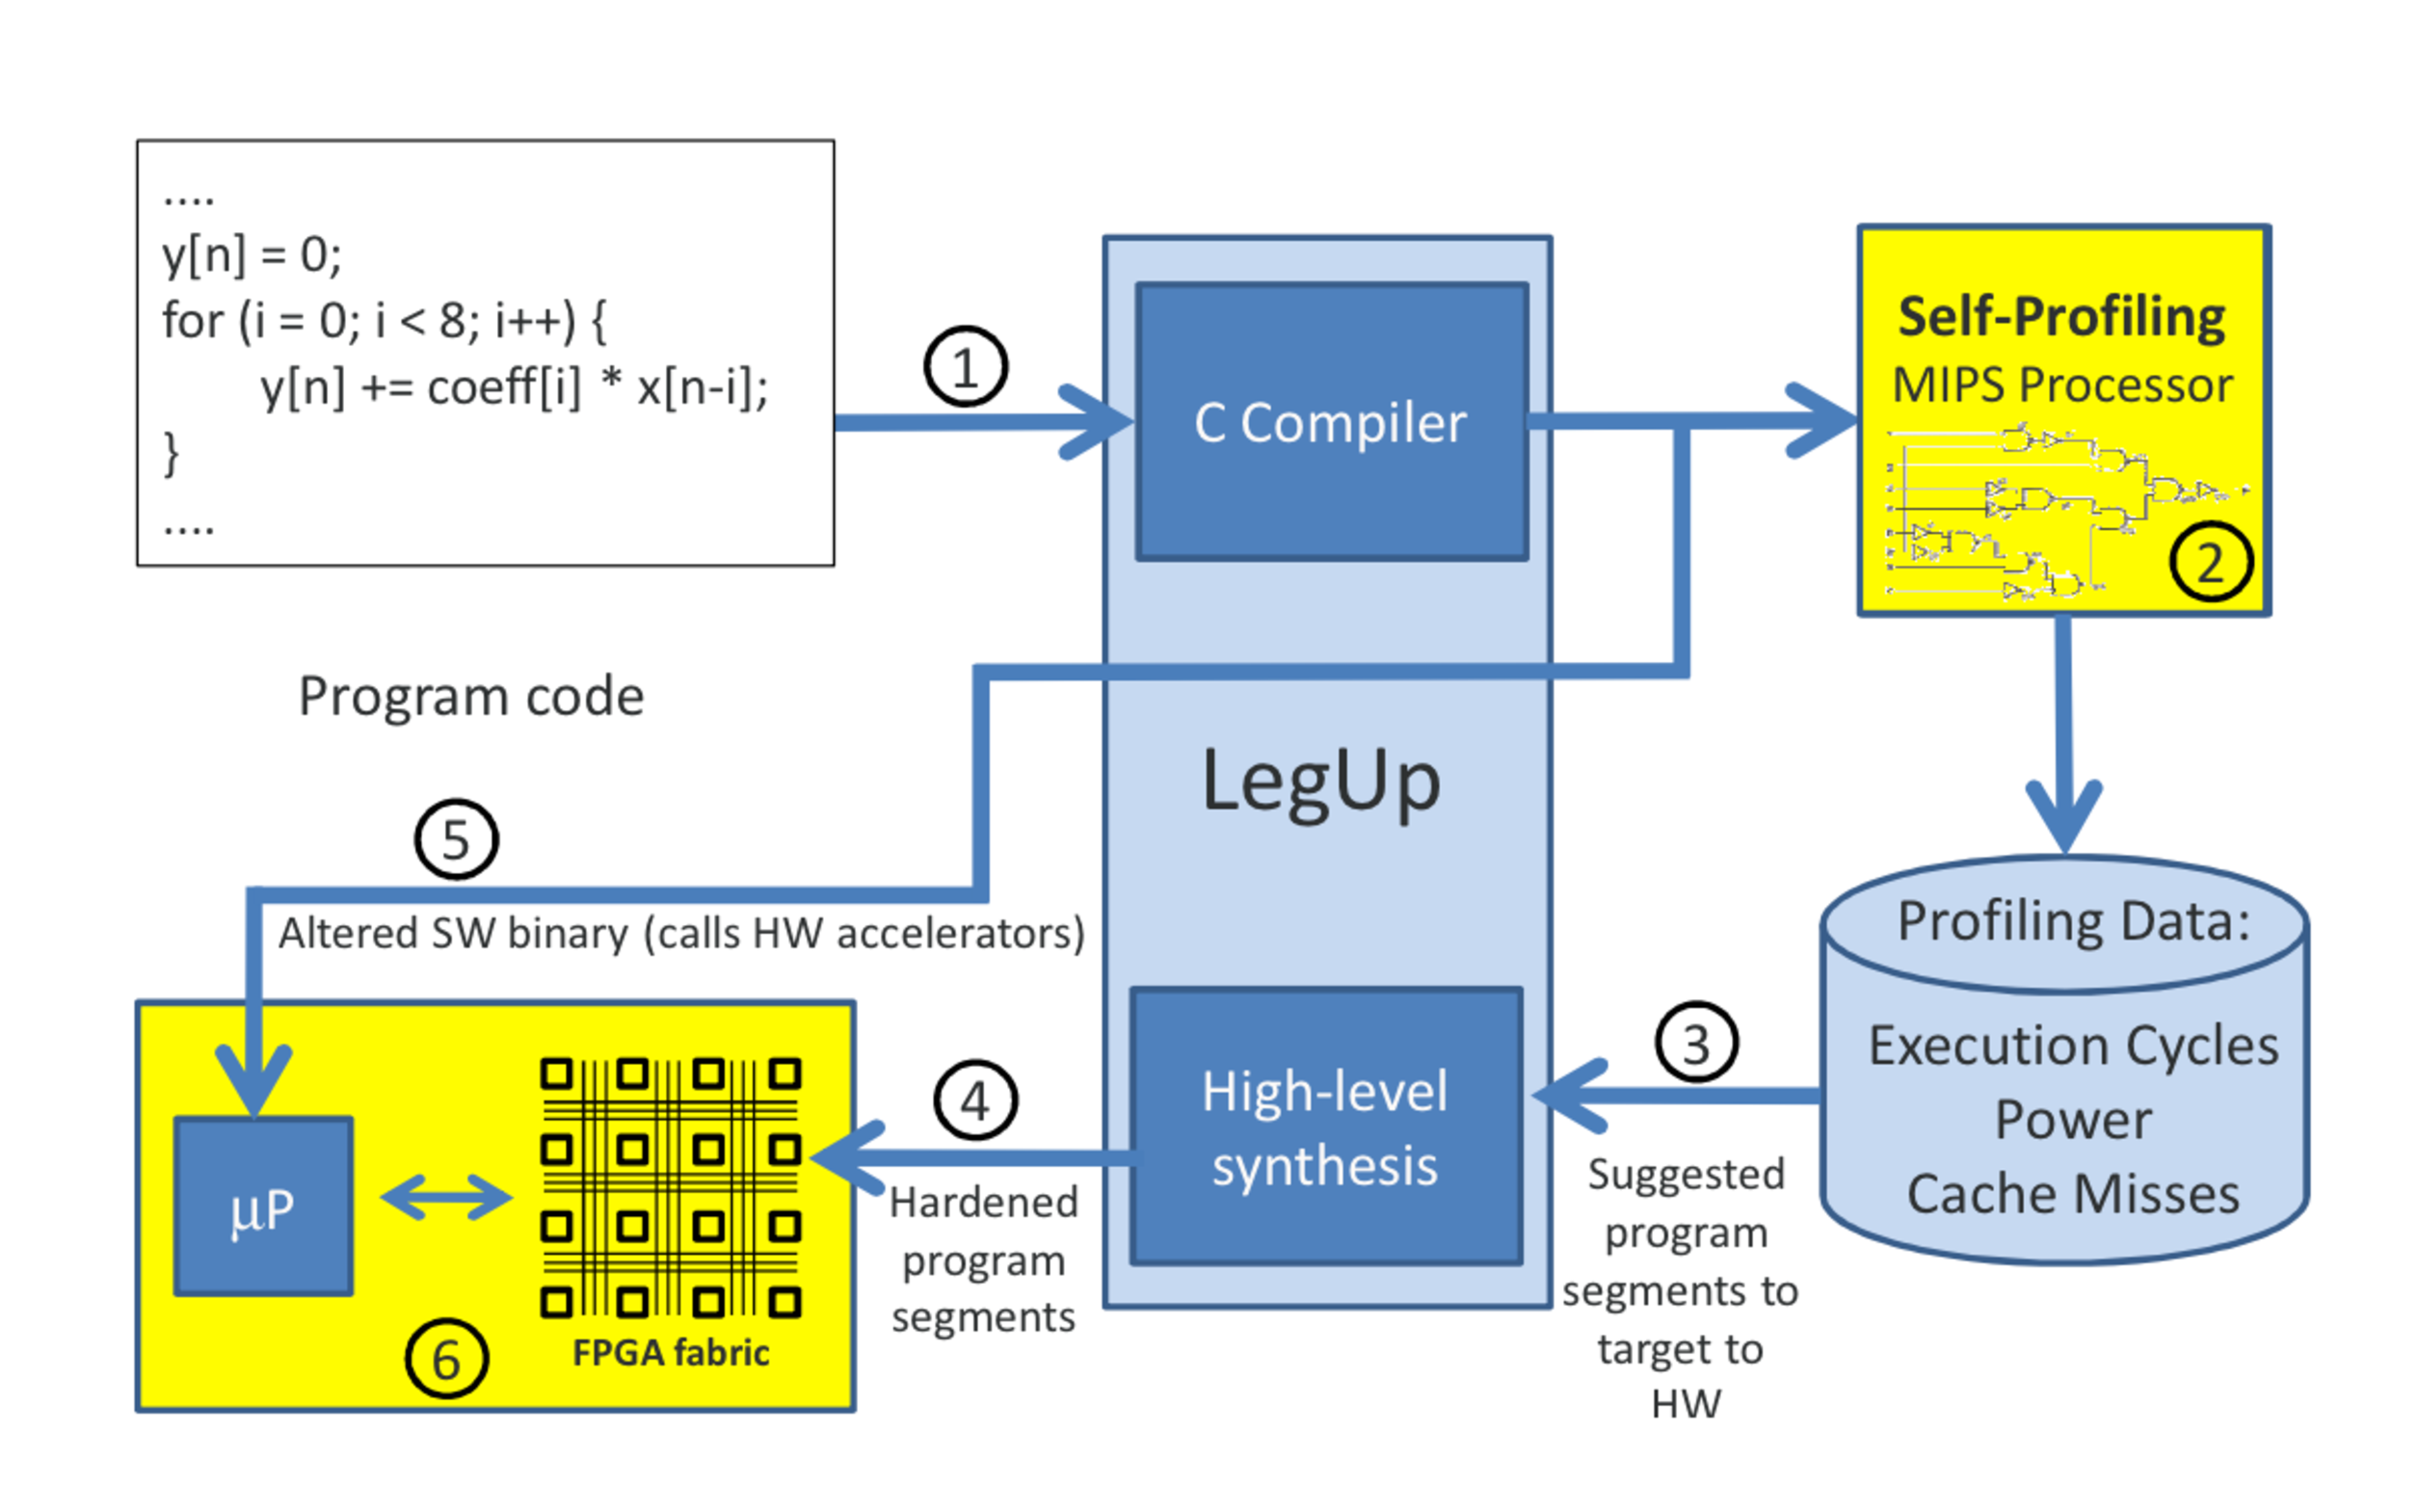
\includegraphics[scale=0.2]{../pictures/legup.pdf}
	      \caption{LegUP \ref{canis2011legup}.}
	      \label{fig:legup}
	    \end{figure}
	  
	  \subsection{Bambu}
	  Bambu\footnote{It can be downloaded at http://panda.dei.polimi.it} is a free framework for the high-level synthesis of complex applications.
	  It takes as input a behavioral description in C and generates as output a Verilog description of the corresponding RTL implementation.
	  \subsection{Modelsim}
	  Well known tool for simulation.
	  
	  \subsection{Cadence}
	  It also supports SystemC simulation.
	\section{Creators and }
	  \subsection{Accellera}
	  Accellera Systems Initiative is a non-profit organization composed of an broad range of members which aims to create system-level standards for the worldwide electronics industry.
	  One of the IEEE\footnote{This standards organization also ratified VHDL, Verilog and SystemVerilog} standards ratified by accellera was IEEE 1666 SystemC.
	  
	\section{Users}
	  \begin{itemize}
	  \item{ARM}
	      \begin{figure}[hp]
		\centering
		
\includegraphics[scale=0.18]{../pictures/armlogo.jpg}
		\caption{ARM Ltd.}
		\label{fig:arm}
	      \end{figure}  
	      ARM (Advanced RISC Machines) Ltd. has an active community\footnote{http://community.arm.com} and there are many informations about tools and IP cores available.
	      SystemC is used by many chip designers and they use the systemC-IP-cores from ARM Ltd. to simulate their designs.
	   \item{AMD}
	   \item{Intel}	    
	   \item{Futjitsu VSLI}	    
	   \item{Casio}	    
	   \item{STMicroelectronics}
	   \item{Realtek}
	  \end{itemize}
\nocite{haubelt2010digitale}
\bibliographystyle{plain}
\bibliography{../references}

\end{document}
